\PassOptionsToPackage{unicode=true}{hyperref} % options for packages loaded elsewhere
\PassOptionsToPackage{hyphens}{url}
\PassOptionsToPackage{dvipsnames,svgnames*,x11names*}{xcolor}
%
\documentclass[]{book}
\usepackage{lmodern}
\usepackage{amssymb,amsmath}
\usepackage{ifxetex,ifluatex}
\usepackage{fixltx2e} % provides \textsubscript
\ifnum 0\ifxetex 1\fi\ifluatex 1\fi=0 % if pdftex
  \usepackage[T1]{fontenc}
  \usepackage[utf8]{inputenc}
  \usepackage{textcomp} % provides euro and other symbols
\else % if luatex or xelatex
  \usepackage{unicode-math}
  \defaultfontfeatures{Ligatures=TeX,Scale=MatchLowercase}
\fi
% use upquote if available, for straight quotes in verbatim environments
\IfFileExists{upquote.sty}{\usepackage{upquote}}{}
% use microtype if available
\IfFileExists{microtype.sty}{%
\usepackage[]{microtype}
\UseMicrotypeSet[protrusion]{basicmath} % disable protrusion for tt fonts
}{}
\IfFileExists{parskip.sty}{%
\usepackage{parskip}
}{% else
\setlength{\parindent}{0pt}
\setlength{\parskip}{6pt plus 2pt minus 1pt}
}
\usepackage{xcolor}
\usepackage{hyperref}
\hypersetup{
            pdftitle={Einführung in die mathematische Datenanalyse},
            pdfauthor={Jan Heiland},
            colorlinks=true,
            linkcolor=Maroon,
            filecolor=Maroon,
            citecolor=Blue,
            urlcolor=purple,
            breaklinks=true}
\urlstyle{same}  % don't use monospace font for urls
\usepackage{color}
\usepackage{fancyvrb}
\newcommand{\VerbBar}{|}
\newcommand{\VERB}{\Verb[commandchars=\\\{\}]}
\DefineVerbatimEnvironment{Highlighting}{Verbatim}{commandchars=\\\{\}}
% Add ',fontsize=\small' for more characters per line
\usepackage{framed}
\definecolor{shadecolor}{RGB}{248,248,248}
\newenvironment{Shaded}{\begin{snugshade}}{\end{snugshade}}
\newcommand{\AlertTok}[1]{\textcolor[rgb]{0.94,0.16,0.16}{#1}}
\newcommand{\AnnotationTok}[1]{\textcolor[rgb]{0.56,0.35,0.01}{\textbf{\textit{#1}}}}
\newcommand{\AttributeTok}[1]{\textcolor[rgb]{0.77,0.63,0.00}{#1}}
\newcommand{\BaseNTok}[1]{\textcolor[rgb]{0.00,0.00,0.81}{#1}}
\newcommand{\BuiltInTok}[1]{#1}
\newcommand{\CharTok}[1]{\textcolor[rgb]{0.31,0.60,0.02}{#1}}
\newcommand{\CommentTok}[1]{\textcolor[rgb]{0.56,0.35,0.01}{\textit{#1}}}
\newcommand{\CommentVarTok}[1]{\textcolor[rgb]{0.56,0.35,0.01}{\textbf{\textit{#1}}}}
\newcommand{\ConstantTok}[1]{\textcolor[rgb]{0.00,0.00,0.00}{#1}}
\newcommand{\ControlFlowTok}[1]{\textcolor[rgb]{0.13,0.29,0.53}{\textbf{#1}}}
\newcommand{\DataTypeTok}[1]{\textcolor[rgb]{0.13,0.29,0.53}{#1}}
\newcommand{\DecValTok}[1]{\textcolor[rgb]{0.00,0.00,0.81}{#1}}
\newcommand{\DocumentationTok}[1]{\textcolor[rgb]{0.56,0.35,0.01}{\textbf{\textit{#1}}}}
\newcommand{\ErrorTok}[1]{\textcolor[rgb]{0.64,0.00,0.00}{\textbf{#1}}}
\newcommand{\ExtensionTok}[1]{#1}
\newcommand{\FloatTok}[1]{\textcolor[rgb]{0.00,0.00,0.81}{#1}}
\newcommand{\FunctionTok}[1]{\textcolor[rgb]{0.00,0.00,0.00}{#1}}
\newcommand{\ImportTok}[1]{#1}
\newcommand{\InformationTok}[1]{\textcolor[rgb]{0.56,0.35,0.01}{\textbf{\textit{#1}}}}
\newcommand{\KeywordTok}[1]{\textcolor[rgb]{0.13,0.29,0.53}{\textbf{#1}}}
\newcommand{\NormalTok}[1]{#1}
\newcommand{\OperatorTok}[1]{\textcolor[rgb]{0.81,0.36,0.00}{\textbf{#1}}}
\newcommand{\OtherTok}[1]{\textcolor[rgb]{0.56,0.35,0.01}{#1}}
\newcommand{\PreprocessorTok}[1]{\textcolor[rgb]{0.56,0.35,0.01}{\textit{#1}}}
\newcommand{\RegionMarkerTok}[1]{#1}
\newcommand{\SpecialCharTok}[1]{\textcolor[rgb]{0.00,0.00,0.00}{#1}}
\newcommand{\SpecialStringTok}[1]{\textcolor[rgb]{0.31,0.60,0.02}{#1}}
\newcommand{\StringTok}[1]{\textcolor[rgb]{0.31,0.60,0.02}{#1}}
\newcommand{\VariableTok}[1]{\textcolor[rgb]{0.00,0.00,0.00}{#1}}
\newcommand{\VerbatimStringTok}[1]{\textcolor[rgb]{0.31,0.60,0.02}{#1}}
\newcommand{\WarningTok}[1]{\textcolor[rgb]{0.56,0.35,0.01}{\textbf{\textit{#1}}}}
\usepackage{longtable,booktabs}
% Fix footnotes in tables (requires footnote package)
\IfFileExists{footnote.sty}{\usepackage{footnote}\makesavenoteenv{longtable}}{}
\usepackage{graphicx,grffile}
\makeatletter
\def\maxwidth{\ifdim\Gin@nat@width>\linewidth\linewidth\else\Gin@nat@width\fi}
\def\maxheight{\ifdim\Gin@nat@height>\textheight\textheight\else\Gin@nat@height\fi}
\makeatother
% Scale images if necessary, so that they will not overflow the page
% margins by default, and it is still possible to overwrite the defaults
% using explicit options in \includegraphics[width, height, ...]{}
\setkeys{Gin}{width=\maxwidth,height=\maxheight,keepaspectratio}
\setlength{\emergencystretch}{3em}  % prevent overfull lines
\providecommand{\tightlist}{%
  \setlength{\itemsep}{0pt}\setlength{\parskip}{0pt}}
\setcounter{secnumdepth}{5}
% Redefines (sub)paragraphs to behave more like sections
\ifx\paragraph\undefined\else
\let\oldparagraph\paragraph
\renewcommand{\paragraph}[1]{\oldparagraph{#1}\mbox{}}
\fi
\ifx\subparagraph\undefined\else
\let\oldsubparagraph\subparagraph
\renewcommand{\subparagraph}[1]{\oldsubparagraph{#1}\mbox{}}
\fi

% set default figure placement to htbp
\makeatletter
\def\fps@figure{htbp}
\makeatother

\usepackage[]{natbib}
\bibliographystyle{plainnat}

\title{Einführung in die mathematische Datenanalyse}
\author{Jan Heiland}
\providecommand{\institute}[1]{}
\institute{FAU Erlangen-Nürnberg}
\date{FAU Erlangen-Nürnberg -- Sommersemester 2022}

\usepackage{amsthm}
\newtheorem{theorem}{Theorem}[chapter]
\newtheorem{lemma}{Lemma}[chapter]
\newtheorem{corollary}{Corollary}[chapter]
\newtheorem{proposition}{Proposition}[chapter]
\newtheorem{conjecture}{Conjecture}[chapter]
\theoremstyle{definition}
\newtheorem{definition}{Definition}[chapter]
\theoremstyle{definition}
\newtheorem{example}{Example}[chapter]
\theoremstyle{definition}
\newtheorem{exercise}{Exercise}[chapter]
\theoremstyle{definition}
\newtheorem{hypothesis}{Hypothesis}[chapter]
\theoremstyle{remark}
\newtheorem*{remark}{Remark}
\newtheorem*{solution}{Solution}
\begin{document}
\maketitle

{
\hypersetup{linkcolor=}
\setcounter{tocdepth}{1}
\tableofcontents
}
\hypertarget{vorwort}{%
\chapter*{Vorwort}\label{vorwort}}
\addcontentsline{toc}{chapter}{Vorwort}

Das ist ein Aufschrieb.

Korrekturen und Wünsche immer gerne als \emph{issues} oder \emph{pull requests} ans \href{https://github.com/highlando/script-emds}{github-repo}.

\hypertarget{was-ist-data-science}{%
\chapter{Was ist Data Science?}\label{was-ist-data-science}}

Data Science umfasst unter anderem folgende Aufgaben:

\begin{enumerate}
\def\labelenumi{\arabic{enumi}.}
\item
  Strukturieren/Aufbereiten (Umgehen mit falschen, korrumpierten, fehlenden,
  unformatierten Daten)
\item
  Data Exploration (Daten ``verstehen'')
\item
  Data Analysis (quantitative Analysen, Hypothesen aufstellen)
\item
  Data Visualization (Hypothesen graphisch kommunizieren)
\item
  Modelle erzeugen/validieren (Regeln/Muster erkennen, Vorhersagen treffen) -- \emph{das} ist Machine Learning aber es gibt auch viele andere Ansätze.
\item
  Daten Reduktion
\end{enumerate}

\hypertarget{wie-passiert-die-datenanalyse}{%
\section{Wie passiert die Datenanalyse?}\label{wie-passiert-die-datenanalyse}}

Mit mathematischen Methoden aus den Bereichen der

\begin{itemize}
\tightlist
\item
  linearen Algebra (z.B. Matrizen, Basen, lineare Gleichungssysteme)
\item
  Statistik (z.B. Mittelwerte, Korrelationen, Verteilungen)
\item
  Analysis (Grenzwerte, Abschätzungen)
\item
  \ldots{}
\end{itemize}

Dabei hilft Software, z.B.,

\begin{itemize}
\tightlist
\item
  Excel
\item
  \textbf{Python}
\item
  Matlab
\item
  R
\end{itemize}

bei der Berechnung, Automatisierung, Visualisierung.

\begin{quote}
Python ist ein de-facto Standard in Data Science und Machine Learning.
\end{quote}

\hypertarget{was-sind-daten}{%
\section{Was sind Daten?}\label{was-sind-daten}}

Wie sehen Daten aus?

\begin{itemize}
\item
  Numerisch reell, z.B. Temperatur
\item
  Numerisch diskret, z.B. Anzahl
\item
  Ordinal: Element einer festen Menge mit expliziter Ordnung, z.B.
  \{neuwertig, mit Gebrauchsspuren, defekt\}
\item
  Binär: Eine von zwei Möglichkeiten, z.B. Wahr/Falsch oder aktiv/inaktiv
\item
  Kategoriell: Element einer festen Menge ohne klare Ordnung, z.B.
  \{Säugetier, Vogel, Fisch\}
\item
  sonstige strukturierte Daten, z.B. geographische Daten, Graphen
\item
  reiner Text, z.B. Freitext in Restaurantbewertung
\end{itemize}

Außerdem können wir noch allgemeine Eigenschaften (Qualitätsmerkmale) von Daten unterscheiden

\begin{itemize}
\tightlist
\item
  strukturiert
\item
  lückenhaft
\item
  fehlerbehaftet (\emph{verrauscht})
\item
  interpretierbar
\item
  geordnet (oder nicht zu ordnen)
\end{itemize}

\hypertarget{beispiele}{%
\section{Beispiele}\label{beispiele}}

\hypertarget{tabellendaten-mietpreise}{%
\subsection{Tabellendaten -- Mietpreise}\label{tabellendaten-mietpreise}}

\begin{figure}
\centering
\includegraphics{bilder/dataframe.png}
\caption{Abbildung: Tabelle von Wohnungsangeboten}
\end{figure}

Hier wären die Aufgaben von Data Science:

\begin{itemize}
\tightlist
\item
  Daten ``verstehen'', Zusammenhänge zwischen
  Variablen aufdecken,
\item
  visualisieren.
\item
  Gegebenenfalls fehlende Einträge bei (z.B.) \texttt{kaltmiete} vorhersagen
\end{itemize}

\begin{figure}
\centering
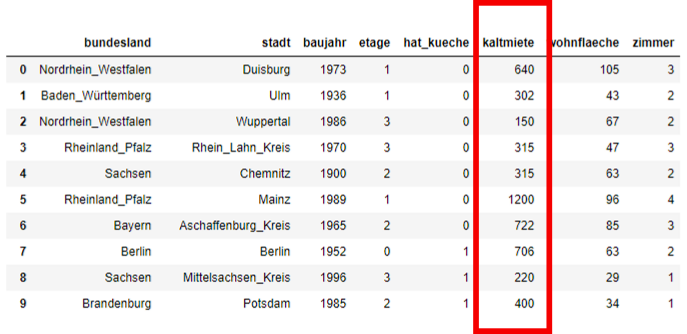
\includegraphics{bilder/dataframe_spalte.png}
\caption{Abbildung: Eine Spalte der Tabelle}
\end{figure}

Datenexploration und -analyse für einzelne Variablen 1/3 Wir betrachten
eine \emph{numerische} Variable in einem rechteckigen Datensatz, also eine
\emph{Spalte} (z.B. \texttt{kaltmiete}). Wir bezeichnen den \(i\)-ten Eintrag in
dieser Spalte mit \(x_i\), wobei \(i=1,\ldots,N\) (\(N\) Anzahl der Zeilen).

Folgende \emph{Schätzer}/\emph{Metriken} können dabei helfen, diese Spalte besser
zu verstehen:

\begin{itemize}
\item
  Mittelwert \(\overline x= \frac1 N\sum_{i=1}^N x_i\)
\item
  gewichteter Mittelwert
  \(\overline x_w = \frac{\sum_{i=1}^N w_i x_i}{\sum_{j=1}^N w_j}\),
  wobei \(w_i\) das Gewicht des \(i\)-ten Eintrages ist (z.B. eine andere
  Variable).
\item
  Varianz: \(s_x^2 = \frac{1}{N-1} \sum_{i=1}^N (x_i-\overline x)^2\)
\item
  Standardabweichung \(s = \sqrt{s_x^2}\).
\item
  Median = \(\frac{315 + 400}{2} = 357.5\).
\end{itemize}

Datenexploration und -analyse für mehrere Variablen Wir betrachten zwei
Spalten \(x = (x_1,\ldots,x_N)\) und \(y = (y_1,\ldots, y_N)\).\\

Das Verteilung von zwei Variablen läßt sich im sogenannte \textbf{Scatter Plot} visualisieren.

\includegraphics[width=0.27\textwidth,height=\textheight]{bilder/dataframe_spalte3.png}
\includegraphics[width=0.7\textwidth,height=\textheight]{bilder/scatterplot.png}

Datenexploration und -analyse für mehrere Variablen Wir betrachten zwei
Spalten \(x = (x_1,\ldots,x_N)\) und \(y = (y_1,\ldots, y_N)\).

\begin{itemize}
\item
  Kovarianz
  \(s_{xy} = \frac{1}{N-1}\sum_{i=1}^N (x_i - \overline x)(y_i - \overline y)\)
\item
  Korrelation \(\rho_{xy} = \frac{s_{xy}}{s_x\cdot s_y} \in [-1,1]\).
\item
  \(\rho \approx 1\): Starke positive Korrelation, wenn \(x\) groß ist,
  ist \(y\) auch groß.
\item
  \(\rho \approx -1\): Starke negative Korrelation, wenn \(x\) groß ist,
  ist \(y\) klein
\item
  \(\rho \approx 0\): Wenig/keine Korrelation.
\end{itemize}

\begin{figure}
\centering
\includegraphics[width=0.65\textwidth,height=\textheight]{bilder/Correlation_coefficient.png}
\caption{Von Kiatdd - Eigenes Werk, CC BY-SA 3.0, \url{https://commons.wikimedia.org/w/index.php?curid=37108966}}
\end{figure}

\hypertarget{covid-19-daten}{%
\subsection{COVID-19 Daten}\label{covid-19-daten}}

Vergleiche die Einführung in \emph{Mathematik für Data Science 1} vom letzten Semester.

\hypertarget{netflix-prize}{%
\subsection{Netflix Prize}\label{netflix-prize}}

Hierbei geht es darum, ob aus bekannten Bewertungen von vielen verschiedenen Benutzern für viele verschiedene Filme abgeleitet werden kann, ob ein bestimmter Nutzer einen bestimmten Film mag (also positiv bewerten würde).

Vergleiche auch \href{https://en.wikipedia.org/wiki/Netflix_Prize}{Wikipedia:Netflix\_Prize}

Das (Trainings-)Daten bestehen über \texttt{480189} Benutzer, die für \texttt{17770} Filme insgesamt \texttt{100480507} Bewertungen als ganze Zahlen zwischen \texttt{1} und \texttt{5} verteilten.

Ziel der Datenanalyse war es, für \texttt{2817131} ``Paare'' von Benutzern und Filmen, die Bewertung vorauszusagen. Neben der schieren Masse an Daten kamen noch Einschränkungen hinzu, die ein Mindestmaß an Qualität der Vorhersage sicherstellen sollten.

Das Problem ließe sich wie folgt darstellen.

\begin{longtable}[]{@{}cccccc@{}}
\toprule
Benutzer \textbackslash{} Film & \texttt{F1} & \texttt{F2} & \texttt{...} & \texttt{Fn} & \texttt{...}\tabularnewline
\midrule
\endhead
\texttt{B1} & -- & 3 & \texttt{...} & 5 & \texttt{...}\tabularnewline
\texttt{B2} & 3 & 4 & \texttt{...} & 2 & \texttt{...}\tabularnewline
\texttt{B3} & 1 & 2 & \texttt{...} & \textbf{?} & \texttt{...}\tabularnewline
\texttt{...} & 3 & 4 & \texttt{...} & -- & \texttt{...}\tabularnewline
\bottomrule
\end{longtable}

Gegeben viele (aber bei weitem nicht alle) Einträge in einer riesigen Tabelle. Können wir aus den Zusammenhängen bestimmte fehlende Einträge (z.B. wie findet Nutzer \texttt{B3} den Film \texttt{Fn}) herleiten?

Die besten Lösungen für dieses Problem basieren durchweg auf \emph{Machine Learning} Ansätzen.

\hypertarget{python}{%
\section{Python}\label{python}}

Die Programmiersprache \texttt{python} wird uns durchs Semester begleiten. Einfach weil sie so wichtig ist für \emph{Data Science} aber auch weil sie (meiner Meinung nach) einfach zu erlernen und zu benutzen ist.

\hypertarget{aufgaben}{%
\section{Aufgaben}\label{aufgaben}}

\hypertarget{python-1}{%
\subsection{Python}\label{python-1}}

Bringen sie ihr \texttt{python} zum Laufen, installieren sie \texttt{numpy}, \texttt{scipy} und \texttt{matplotlib} und führen sie das folgende script aus.

\begin{Shaded}
\begin{Highlighting}[]
\ImportTok{import}\NormalTok{ numpy }\ImportTok{as}\NormalTok{ np}
\ImportTok{import}\NormalTok{ matplotlib.pyplot }\ImportTok{as}\NormalTok{ plt}

\NormalTok{N }\OperatorTok{=} \DecValTok{20}
\NormalTok{xmax }\OperatorTok{=} \DecValTok{2}
\NormalTok{xmin }\OperatorTok{=} \DecValTok{0}

\NormalTok{xdata }\OperatorTok{=}\NormalTok{ np.linspace(xmin, xmax, N)}
\NormalTok{ydata }\OperatorTok{=}\NormalTok{ np.exp(xdata)}

\NormalTok{plt.figure(}\DecValTok{1}\NormalTok{)}
\NormalTok{plt.plot(xdata, ydata, }\StringTok{'.'}\NormalTok{)}

\NormalTok{plt.figure(}\DecValTok{2}\NormalTok{)}
\NormalTok{plt.semilogy(xdata, ydata, }\StringTok{'.'}\NormalTok{)}
\NormalTok{plt.show()}
\end{Highlighting}
\end{Shaded}

\hypertarget{einheitsmatrix}{%
\subsection{Einheitsmatrix}\label{einheitsmatrix}}

Schreiben sie ein script, dass die \texttt{5x5} Einheitsmatrix auf 3 verschiedene Arten erzeugt. (Eine Art könnte die eingebaute \texttt{numpy} Funktion \texttt{eye} sein).

\begin{Shaded}
\begin{Highlighting}[]
\ImportTok{import}\NormalTok{ numpy }\ImportTok{as}\NormalTok{ np}

\NormalTok{idfive }\OperatorTok{=}\NormalTok{ np.eye(}\DecValTok{5}\NormalTok{)}
\BuiltInTok{print}\NormalTok{(idfive)}
\end{Highlighting}
\end{Shaded}

Hinweis: schauen sie sich mal an wie \texttt{numpy}'s \texttt{arrays} funktionieren.

\hypertarget{matrizen-multiplikation-und-potenz}{%
\subsection{Matrizen Multiplikation und Potenz}\label{matrizen-multiplikation-und-potenz}}

Schreiben sie ein script, das die Übungsaufgabe aus der Vorlesung (potenzieren der Matrizen \(M_i\), \(i=1,2,3,4\)) löst. Zum Beispiel mit

\begin{Shaded}
\begin{Highlighting}[]
\ImportTok{import}\NormalTok{ numpy }\ImportTok{as}\NormalTok{ np}
\NormalTok{mone }\OperatorTok{=}\NormalTok{ np.array([[}\FloatTok{0.9}\NormalTok{, }\FloatTok{0.9}\NormalTok{], [}\FloatTok{0.9}\NormalTok{, }\FloatTok{0.9}\NormalTok{]])}

\NormalTok{mone_ptwo }\OperatorTok{=}\NormalTok{ mone }\OperatorTok{@}\NormalTok{ mone}
\BuiltInTok{print}\NormalTok{(mone_ptwo)}

\NormalTok{mone_pfour }\OperatorTok{=}\NormalTok{ mone_ptwo }\OperatorTok{@}\NormalTok{ mone_ptwo}
\BuiltInTok{print}\NormalTok{(mone_pfour)}
\end{Highlighting}
\end{Shaded}

Oder so:

\begin{Shaded}
\begin{Highlighting}[]
\ImportTok{import}\NormalTok{ numpy }\ImportTok{as}\NormalTok{ np}
\NormalTok{mone }\OperatorTok{=}\NormalTok{ np.array([[}\FloatTok{0.9}\NormalTok{, }\FloatTok{0.9}\NormalTok{], [}\FloatTok{0.9}\NormalTok{, }\FloatTok{0.9}\NormalTok{]])}
\NormalTok{mone_p }\OperatorTok{=}\NormalTok{ np.eye(}\DecValTok{2}\NormalTok{)}

\ControlFlowTok{for}\NormalTok{ k }\KeywordTok{in} \BuiltInTok{range}\NormalTok{(}\DecValTok{16}\NormalTok{):}
\NormalTok{    mone_p }\OperatorTok{=}\NormalTok{ mone_p }\OperatorTok{@}\NormalTok{ mone}
    \ControlFlowTok{if}\NormalTok{ k }\OperatorTok{==} \DecValTok{1} \KeywordTok{or}\NormalTok{ k }\OperatorTok{==} \DecValTok{3} \KeywordTok{or}\NormalTok{ k }\OperatorTok{==} \DecValTok{15}\NormalTok{:}
        \BuiltInTok{print}\NormalTok{(}\StringTok{'k='}\NormalTok{, k}\OperatorTok{+}\DecValTok{1}\NormalTok{)}
        \BuiltInTok{print}\NormalTok{(mone_p)}
\end{Highlighting}
\end{Shaded}

Achtung:

\begin{itemize}
\tightlist
\item
  bei Matrizen kann auch \texttt{*} benutzt werden -- das ist aber nicht die richtige Matrizenmultiplikation (sondern die Multiplikation eintragsweise)
\item
  Moegliche Realisierung der Matrizenmultiplikation

  \begin{itemize}
  \tightlist
  \item
    \texttt{np.dot(A,\ B)} -- die klassische Methode
  \item
    \texttt{A.dot(B)} -- das selbe (manchmal besser, wenn \texttt{A} etwas allgemeiner ist (zum Beispiel eine \texttt{scipy.sparse} matrix)
  \item
    \texttt{A\ @\ B} -- convenience Notation
  \end{itemize}
\end{itemize}

\hypertarget{lineare-regression}{%
\chapter{Lineare Regression}\label{lineare-regression}}

Auch bekannt als

\begin{itemize}
\tightlist
\item
  \emph{lineare Ausgleichsrechnung} oder
\item
  \emph{Methode der kleinsten Quadrate}.
\end{itemize}

Ein wesentlicher Aspekt von \emph{Data Science} ist die Analyse oder das
Verstehen von Daten. Allgemein gesagt, es wird versucht, aus den Daten
heraus Aussagen über Trends oder Eigenschaften des Phänomens zu treffen,
mit welchem die Daten im Zusammenhang stehen.

Wir kommen nochmal auf das Beispiel aus der Einführungswoche zurück, werfen eine bereits geschärften Blick darauf und gehen das mit verbesserten mathematischen Methoden an.

Gegeben seien die Fallzahlen aus der CoVID Pandemie 2020 für Bayern für den Oktober 2020.

\hypertarget{tab:covid-cases}{}
\begin{longtable}[]{@{}llllllllllll@{}}
\caption{Anzahl der SARS-CoV-2 Neuinfektionen in Bayern im Oktober 2020.}\tabularnewline
\toprule
Tag & 1 & 2 & 3 & 4 & 5 & 6 & 7 & 8 & 9 & 10 & 11\tabularnewline
\midrule
\endfirsthead
\toprule
Tag & 1 & 2 & 3 & 4 & 5 & 6 & 7 & 8 & 9 & 10 & 11\tabularnewline
\midrule
\endhead
Fälle & 352 & 347 & 308 & 151 & 360 & 498 & 664 & 686 & 740 & 418 & 320\tabularnewline
\bottomrule
\end{longtable}

\begin{longtable}[]{@{}lllllllllll@{}}
\toprule
Tag & 12 & 13 & 14 & 15 & 16 & 17 & 18 & 19 & 20 & 21\tabularnewline
\midrule
\endhead
Fälle & 681 & 691 & 1154 & 1284 & 127 & 984 & 573 & 1078 & 1462 & 2239\tabularnewline
\bottomrule
\end{longtable}

\begin{longtable}[]{@{}lllllllllll@{}}
\toprule
Tag & 22 & 23 & 24 & 25 & 26 & 27 & 28 & 29 & 30 & 31\tabularnewline
\midrule
\endhead
Fälle & 2236 & 2119 & 1663 & 1413 & 2283 & 2717 & 3113 & 2972 & 3136 & 2615\tabularnewline
\bottomrule
\end{longtable}

\begin{figure}
\hypertarget{fig:cases}{%
\centering
\includegraphics{bilder/02-cases.png}
\caption{Fallzahlen von Sars-CoV-2 in Bayern im Oktober
2020}\label{fig:cases}
}
\end{figure}

Wieder stellen wir uns die Frage ob wir \textbf{in den Daten einen funktionalen
Zusammenhang} feststellen können. Also ob wir die Datenpaare

\begin{quote}
(Tag \(x\), Infektionen am Tag \(x\))
\end{quote}

die wir als

\begin{quote}
(\(x_i\), \(y_i\))
\end{quote}

über eine Funktion \(f\) und die Paare

\begin{quote}
(\(x\), \(f(x)\))
\end{quote}

beschreiben (im Sinne von gut darstellen oder approximieren) können.

\hypertarget{rauschen-und-fitting}{%
\section{Rauschen und Fitting}\label{rauschen-und-fitting}}

Beim obigen Beispiel (und ganz generell bei Daten) ist davon auszugehen, dass die Daten \textbf{verrauscht} sind, also einem Trend folgen oder in einem funktionalen Zusammenhang stehen aber zufällige Abweichungen oder Fehler enthalten.

Unter diesem Gesichtspunkt ist eine Funktion, die

\begin{quote}
\(f(x_i)=y_i\)
\end{quote}

erzwingt nicht zielführend. (Wir wollen Trends und größere Zusammenhänge erkennen und nicht kleine Fehler nachzeichnen.) Das zu strenge Anpassen an möglicherweise verrauschte Daten wird \textbf{overfitting} genannt.

Vielmehr werden wir nach einer Funktion \(f\) suchen, die die Daten näherungsweise nachstellt:

\begin{quote}
\(f(x_i)\approx y_i\)
\end{quote}

Hierbei passen jetzt allerdings auch Funktionen, die vielleicht einfach zu handhaben sind aber die Daten kaum noch repräsentieren. Jan spricht von \textbf{underfitting}.

Eine gute Approximation besteht im Kompromiss von \emph{nah an den Daten} aber mit wenig \emph{overfitting}.

\hypertarget{ansuxe4tze-fuxfcr-lineare-regression}{%
\section{Ansätze für lineare Regression}\label{ansuxe4tze-fuxfcr-lineare-regression}}

Um eine solche Funktion \(f\) zu finden, trifft Jan als erstes ein paar
Modellannahmen. Modellannahmen legen fest, wie das \(f\) im Allgemeinen
aussehen soll und versuchen dabei

\begin{enumerate}
\def\labelenumi{\arabic{enumi}.}
\item
  die Bestimmung von \(f\) zu ermöglichen
\item
  zu garantieren, dass \(f\) auch die gewollten Aussagen liefert
\item
  und sicherzustellen, dass \(f\) zum Problem passt.
\end{enumerate}

Jan bemerke, dass die ersten beiden Annahmen im Spannungsverhältnis zur
dritten stehen.

\textbf{Lineare Regression} besteht darin, dass die Funktion als Linearkombination

\begin{equation*}
f_w(x) = \sum_{j=1}^n w_j b_j(x)
\end{equation*}

von Basisfunktionen geschrieben wird und dann die \emph{Koeffizienten} \(w_i\) so bestimmt werden, dass \(f\) die Daten bestmöglich annähert.

\begin{quote}
Jan bemerke, dass \emph{bestmöglich} wieder \emph{overfitting} bedeuten kann aber auch, bei schlechter Wahl der Basis, wenig aussagekräftig sein kann. Der gute Kompromiss liegt also jetzt in der Wahl der passenden Basisfunktionen und deren Anzahl. (Mehr Basisfunktionen bedeutet möglicherweise bessere Approximation aber auch die Gefahr von \emph{overfitting}.)
\end{quote}

Typische Wahlen für die Basis \(\{b_1, b_2, \dotsc, b_n\}\) sind

\begin{itemize}
\tightlist
\item
  Polynome: \(\{1, x, x^2, \dotsc, x^{n-1}\}\) -- für \(n=2\) ist der Ansatz \emph{eine Gerade}
\item
  Trigonometrische Funktionen: \(\{1, \cos(x), \sin(x), \cos(2x), \sin(2x), \dotsc\}\)
\item
  Splines -- Polynome, die abschnittsweise definiert werden
\item
  Wavelets -- Verallgemeinerungen von trigonometrischen Funktionen
\end{itemize}

\hypertarget{fehlerfunktional-und-minimierung}{%
\section{Fehlerfunktional und Minimierung}\label{fehlerfunktional-und-minimierung}}

Wir setzen nun also an
\begin{equation*}
f_w(x) = \sum_{j=1}^nw_j b_j (x)
\end{equation*}
und wollen damit \(y_i \approx f_w(x_i)\) \emph{bestmöglich} erreichen (indem wir die Koeffizienten \((w_1, \dotsc, w_n)\) \emph{optimal} wählen. Bestmöglich und optimal spezifizieren wir über den Mittelwert der quadratischen Abweichungen in der Approximation über alle Datenpunkte
\begin{equation*}
\frac{1}{N}\sum_{i=1}^N (y_i - f_w(x_i))^2
\end{equation*}

Ein paar Bemerkungen

\begin{itemize}
\tightlist
\item
  jetzt müssen wir die \(w_i\)'s bestimmen so dass dieser Fehlerterm minimal wird
\item
  das optimale \(w\) ist unabhängig von einer Skalierung des Fehlerterms
\item
  des wegen schreiben wir gerne einfach \(\frac 12 \sum_{i=1}^N (y_i - f_w(x_i))^2\) als das Zielfunktional, das es zu minimieren gilt.
\end{itemize}

Wie finden wir jetzt die \(w_i\)'s? Zunächst gilt, dass
\begin{equation*}
f_w(x_i) = \sum_{i=j}^n w_j b_j(x_i) = 
\begin{bmatrix}
b_1(x_i) & b_2(x_i) & \dots & b_n(x_i)
\end{bmatrix}
\begin{bmatrix}
w_1 \\ w_2 \\ \vdots \\ w_n
\end{bmatrix}
\end{equation*}

und wenn wir alle \(f_w(x_i)\), \(i=1,\dotsc,N\) übereinander in einen Vektor schreiben, dass

\begin{equation*}
f_w(\mathbf x) := 
\begin{bmatrix}
f_w(x_1) \\ \vdots \\ f_w(x_N)
\end{bmatrix}
=
\begin{bmatrix}
b_1(x_1) & \dots & b_n(x_1) \\
\vdots & \ddots & \vdots \\
b_1(x_N) & \dots & b_n(x_N)
\end{bmatrix}
\begin{bmatrix}
w_1 \\ \vdots \\ w_n
\end{bmatrix}
=: \Phi(\mathbf x) w
\end{equation*}

Damit, mit \(\mathbf y\) als den Vektor aller \(y_i\)'s, und mit der Definition der Vektornorm, können wir unser Minimierungsproblem schreiben als
\begin{equation*}
\frac 12  \sum_{i=1}^N (y_i - f_w(x_i))^2 = \frac 12 \| \mathbf y - \Phi (\mathbf x) w\|^2 \to \min.
\end{equation*}

Wir bemerken, dass

\begin{itemize}
\tightlist
\item
  das Fehlerfunktional immer größer und bestenfalls gleich 0 ist
\item
  falls das lineare Gleichungssystem \(\Phi (\mathbf x)w = \mathbf y\) eine Lösung \(w\) hat, ist das auch eine Lösung unserer Minimierung
\item
  im typischen Falle aber ist allerdings \(N\gg n\) und das System überbestimmt (\(n=N\) würde ein overfitting bedeuten\ldots{}) sodass wir keine Lösung des linearen Gleichungssystems erwarten können.
\item
  Das Minimierungsproblems selbst hat allerdings immer eine Lösung.
\end{itemize}

\hypertarget{berechnung-der-bestluxf6sung}{%
\section{Berechnung der Bestlösung}\label{berechnung-der-bestluxf6sung}}

Wir suchen also ein Minimum der Funktion (mit \(\Phi\), \(\mathbf x\), \(\mathbf y\) gegeben)
\begin{equation*}
\begin{split}
w \mapsto \frac 12 \|\mathbf y - \Phi(\mathbf x)w \|^2 &= \frac 12 (\mathbf y - \Phi(\mathbf x)w)^T(\mathbf y - \Phi(\mathbf x)w)  \\ 
&= \frac 12 [\mathbf y^T\mathbf y - \mathbf y^T \Phi(\mathbf x)w - w^T \Phi(\mathbf x)^T\mathbf y  + w^T \Phi(\mathbf x)^T\Phi(\mathbf x)w] \\
&= \frac 12 [\mathbf y^T\mathbf y -2 w^T \Phi(\mathbf x)^T\mathbf y  + w^T \Phi(\mathbf x)^T\Phi(\mathbf x)w] 
\end{split}
\end{equation*}
wobei wir die Definition der Norm \(\|v\|^2 = v^Tv\) und die Eigenschaft, dass für die skalare Größe \(w^T \Phi(\mathbf x)^T\mathbf y = [w^T \Phi(\mathbf x)^T\mathbf y]^T = \mathbf y^T \Phi(\mathbf x)w\) gilt, ausgenutzt haben.

Wären \(w\) und \(\mathbf y\) keine Vektoren sondern einfach reelle Zahlen, wäre das hier eine Parabelgleichung \(aw^2 + bw + c\) mit \(a>0\), die immer eine Minimalstelle hat.

Tatsächlich gilt hier alles ganz analog. Insbesondere ist \(\Phi(\mathbf x)^T\Phi(\mathbf x)\) in der Regel ``größer 0'' (was heißt das wohl bei quadratischen Matrizen?). Und mittels ``Nullsetzen'' der ersten Ableitung können wir das Minimum bestimmen. In diesem Fall ist die erste Ableitung (nach \(w\))
\begin{equation*}
\nabla_w (\frac 12 \|\mathbf y - \Phi(\mathbf x) \|^2) = \Phi(\mathbf x)^T\Phi(\mathbf x)w - \Phi(\mathbf x)^T\mathbf y,
\end{equation*}
(den \emph{Gradienten} \(\nabla_w\) als Ableitung von Funktionen mit mehreren Veränderlichen werden wir noch genauer behandeln)
was uns als Lösung, die Lösung des linearen Gleichungssystems
\begin{equation*}
\Phi(\mathbf x)^T\Phi(\mathbf x)w = \Phi(\mathbf x)^T\mathbf y
\end{equation*}
definiert.

Letzte Frage: Wann hat dieses Gleichungssystems eine eindeutige Lösung? Mit \(N>n\) (also \(\Phi(\mathbf x)\) hat mehr Zeilen als Spalten) gelten die Äquivalenzen:

\begin{itemize}
\tightlist
\item
  \(\Phi(\mathbf x)^T\Phi(\mathbf x)w = \Phi(\mathbf x)^T\mathbf y\) hat eine eindeutige Lösung
\item
  die Matrix \(\Phi(\mathbf x)^T\Phi(\mathbf x)\) ist regulär
\item
  die Spalten von \(\Phi(\mathbf x)\) sind linear unabhängig
\item
  die Vektoren \(b_i(\mathbf x)\) sind linear unabhängig.
\end{itemize}

Praktischerweise tritt genau diese Situation im Allgemeinen ein.

\begin{itemize}
\tightlist
\item
  \(N>n\) (mehr Datenpunkte als Parameter)
\item
  \(b_i\)'s werden als \emph{linear unabhängig} (im Sinne ihres Funktionenraums) gewählt, was die lineare unabhängigket der \(b_i(\mathbf x)\) impliziert.
\end{itemize}

\hypertarget{beispiel}{%
\section{Beispiel}\label{beispiel}}

Unsere Covid-Zahlen ``mit einer Geraden angenähert'':

\begin{itemize}
\tightlist
\item
  \(f_w(x) = w_1 + w_2 x\) -- das heißt \(n=2\) und Basisfunktionen \(b_1(x)\equiv 1\) und \(b_2(x) = x\)
\item
  \(\mathbf x = (1,2,3, \dots, 31)\) -- die Tage im Februar, das heißt \(N=31\)
\item
  \(\mathbf y = (352, 347, \dots, 2615)\) -- die Fallzahlen
\end{itemize}

Wir bekommen

\begin{equation*}
\Phi(\mathbf x) = 
\begin{bmatrix}
1 & 1 \\ 1 & 2 \\ 1 & 3 \\ \vdots & \vdots \\ 1 & 31
\end{bmatrix}
\end{equation*}
(die Spalten sind linear unabhängig) und müssen ``nur'' das 2x2 System
\[
\begin{bmatrix}
1 & 1 & 1 & \dots & 1 \\ 1 & 2 & 3 & \dots & 31
\end{bmatrix}
\begin{bmatrix}
1 & 1 \\ 1 & 2 \\ 1 & 3 \\ \vdots \\ 1 & 31
\end{bmatrix}
\begin{bmatrix}
w_1 \\ w_2
\end{bmatrix}
=
\begin{bmatrix}
1 & 1 & 1 & \dots & 1 \\ 1 & 2 & 3 & \dots & 31
\end{bmatrix} 
\begin{bmatrix}
352 \\  347 \\ 308 \\ \vdots \\ 2615
\end{bmatrix} 
\]
lösen um die Approximation \(f_w\) zu bestimmen.

Und noch als letzte Bemerkung. Egal wie die Basisfunktionen \(b_i\) gewählt werden, die Parameterabhängigkeit von \(w\) ist immer linear. Deswegen der Name \textbf{lineare Ausgleichsrechnung}.

\hypertarget{matrix-zerlegungen}{%
\chapter{Matrix-Zerlegungen}\label{matrix-zerlegungen}}

Die Lösung \(w\) des Problems der \emph{linearen Ausgleichsrechnung} war entweder als Lösung eines Optimierungsproblems
\begin{equation*}
\min_{w} \| Aw - y \|^2
\end{equation*}
oder als Lösung des linearen Gleichungssystems
\begin{equation*}
A^TAw=y
\end{equation*}
gegeben. Hierbei steht nun \(A\in \mathbb R^{N\times n}\) für die Matrix \(\Phi(\mathbf x)\) der Daten und Basisfunktionen. Wir hatten uns überlegt, dass in den meisten Fällen

\begin{itemize}
\tightlist
\item
  die Matrix mehr Zeilen als Spalten hat (\(N>n\)) und
\item
  die Spalten linear unabhängig sind.
\end{itemize}

\hypertarget{qr-zerlegung}{%
\section{QR Zerlegung}\label{qr-zerlegung}}

Wir betrachten nochmal das Optimierungsproblem \(\min_{w} \| Aw - y \|^2\). Gäbe es eine Lösung des Systems \(Aw=y\), wäre das sofort eine Lösung des Optimierungsproblems. Da \(A\) aber mehr Zeilen als Spalten hat, ist das System \(Aw=y\) überbestimmt und eine Lösung in der Regel nicht gegeben.

Die Überlegung ist nun, die Gleichung \(Aw=y\) \emph{so gut wie möglich} zu erfüllen, indem wir die relevanten Gleichungen indentifizieren und wenigstens diese lösen. Ein systematischer (und wie wir später sehen werden auch zum Optimierungsproblem passender) Zugang bietet die QR Zerlegung.

\begin{theorem}[QR Zerlegung]
\protect\hypertarget{thm:qr}{}\label{thm:qr}Sei \(A\mathbb R^{m\times n}\), \(m>n\). Dann existiert eine orthonormale Matrix \(Q\in \mathbb R^{m\times m}\) und eine obere Dreiecksmatrix \(\hat R\in \mathbb R^{n\times n}\) derart dass
\begin{equation*}
A = QR =: Q 
\begin{bmatrix}
\hat R \\ 0
\end{bmatrix}.
\end{equation*}
Hat \(A\) vollen (Spalten)Rang, dann ist \(\hat R\) invertierbar.
\end{theorem}

Hier heißt \emph{orthonormale Matrix} \(Q\), dass die Spalten von \(Q\) paarweise orthogonal sind. Insbesondere gilt
\begin{equation*}
Q^T Q = I.
\end{equation*}

Für unser zu lösendes Problem ergibt sich dadurch die Umformung
\begin{equation*}
Aw = y \quad \Leftrightarrow \quad QRw=y \quad \Leftrightarrow \quad Q^TQRw=Q^T y 
 \quad \Leftrightarrow \quad  Rw = Q^Ty
\end{equation*}
oder auch
\begin{equation*}
\begin{bmatrix}
\hat R \\ 0
\end{bmatrix}w 
=
Q^Ty
=
\begin{bmatrix}
Q_1^T \\ Q_2^T
\end{bmatrix}
y
\end{equation*}
(wobei wir die \(Q_1\in \mathbb R^{m\times n}\) die Matrix der ersten \(n\) Spalten von \(Q\) ist)
und als \emph{Kompromiss} der Vorschlag, das Teilsystem
\begin{equation*}
\hat R w = Q_1^Ty
\end{equation*}
nach \(w\) zu lösen und in Kauf zu nehmen, dass der Rest, nämlich das \(Q_2^Ty\), nicht notwendigerweise gleich null ist.

Wir halten zunächst mal fest, dass

\begin{itemize}
\tightlist
\item
  Obwohl \(Q\) eine reguläre Matrix ist, bedarf der Übergang von \(Aw=y\) zu \(Q^TAw=Q^Ty\) einer genaueren Analyse.
\item
  Wir bemerken, dass für eine hypothetische komplette Lösung \(Aw-y\), diese Transformation keine Rolle spielt.
\item
  Für die Kompromisslösung jedoch schon, weil beispielsweise verschiedene Konstruktionen eines invertierbaren Teils, verschiedene Residuen bedeuten und somit Optimalität im Sinne von \(\min_w \|Aw-y\|^2\) nicht garantiert ist.
\end{itemize}

Allerdings, wie Sie als Übungsaufgabe nachweisen werden, löst dieser Ansatz tatsächlich das Optimierungsproblem.

\hypertarget{singuluxe4rwertzerlegung}{%
\section{Singulärwertzerlegung}\label{singuluxe4rwertzerlegung}}

Eine weitere Matrix Zerlegung, die eng mit der Lösung von Optimierungsproblemen oder überbestimmten Gleichungssystemen zusammenhängt ist die \emph{Singulärwertzerlegung} (SVD -- von english: \emph{Singular Value Decomposition}).

\begin{theorem}[Singulärwertzerlegung]
\protect\hypertarget{thm:svd}{}\label{thm:svd}Sei \(A\in \mathbb C^{m\times n}\), \(m\geq n\). Dann existieren orthogonale Matrizen \(U \in \mathbb C^{m\times m}\) und \(V\in \mathbb C^{n\times n}\) und eine Matrix \(\Sigma \in \mathbb R^{m\times n}\) der Form
\begin{equation*}
\Sigma = 
\begin{bmatrix}
\sigma_1 & 0 & \dots & 0\\
0 & \sigma_2 &\ddots & \vdots\\
0 & \ddots & \ddots &0\\
  0 & \dots&0 & \sigma_n \\
  0 & 0 & \dots & 0 \\
  \vdots & \ddots &  & \vdots\\
  0 & 0 & \dots & 0
\end{bmatrix}
\end{equation*}
mit reellen sogenannten \emph{Singulärwerten}
\begin{equation*}
\sigma_1 \geq \sigma_2 \geq \dots \geq \sigma_n \geq 0
\end{equation*}
sodass gilt
\begin{equation*}
A = U \Sigma V^*
\end{equation*}
wobei gilt \(V^* = \overline{V^T}\) (transponiert und komplex konjugiert).
\end{theorem}

Ein paar Bemerkungen.

\begin{itemize}
\tightlist
\item
  Ist \(A\) reell, können auch \(U\) und \(V\) reell gewählt werden.
\item
  Die Annahme \(m \geq n\) war nur nötig um für die Matrix \(\Sigma\) keine Fallunterscheidung zu machen. (Für \(m\leq n\) ``steht der Nullblock rechts von den Singulärwerten''). Insbesondere gilt \(A^* = V\Sigma U^*\) ist eine SVD von \(A^*\).
\item
  Eine Illustration der Zerlegung ist in Abbildung \ref{SVD} zu sehen.
\end{itemize}

Wir machen einige Überlegungen im Hinblick auf große Matrizen. Sei dazu \(m>n\), \(A\in \mathbb C^{m\times n}\) und \(A=U\Sigma V^*\) eine SVD wie in Theorem @ref\{thm:SVD\}. Sei nun
\begin{equation*}
U = \begin{bmatrix}
U_1 & U_2
\end{bmatrix}
% = \begin{bmatrix} V_1^* & V_2^*
\end{equation*}
partitioniert sodass \(U_1\) die ersten \(n\) Spalten von \(U\) enthält.

Dann gilt (nach der Matrix-Multiplikations Regel \emph{Zeile mal Spalte} die Teile \(U_2\) und \(V_2\) immer mit dem Nullblock in \(\Sigma\) multipliziert werden) dass
\begin{equation*}
A = U\Sigma V = 
\begin{bmatrix}
U_1 & U_2
\end{bmatrix}
\begin{bmatrix}
\hat \Sigma \\ 0
\end{bmatrix}
V^*
% \begin{bmatrix} V_1^* \\ V_2^* \end{bmatrix}
=
U_1 
\hat \Sigma
V^*
% \begin{bmatrix} V_1^* \\ V_2^* \end{bmatrix}
\end{equation*}
Es genügt also nur die ersten \(m\) Spalten von \(U\) zu berechnen. Das ist die sogenannte \textbf{slim SVD}.

Hat, darüberhinaus, die Matrix \(A\) keinen vollen Rang, also \(\operatorname{Rg}(A) = r < n\), dann:

\begin{itemize}
\tightlist
\item
  ist \(\sigma_i=0\), für alle \(i=r+1, \dotsc, n\), (wir erinnern uns, dass die Singulärwerte nach Größe sortiert sind)
\item
  die Matrix \(\hat \Sigma\) hat \(n-r\) Nullzeilen
\item
  für die Zerlegung sind nur die ersten \(r\) Spalten von \(U\) und \(V\) relevant -- die sogenannte \textbf{Kompakte SVD}.
\end{itemize}

In der Datenapproximation ist außerdem die \textbf{truncated SVD} von Interesse. Dazu sei \(\hat r<r\) ein beliebig gewählter Index. Dann werden alle Singulärwerte, \(\sigma_i=0\), für alle \(i=\hat r+1, \dotsc, n\), abgeschnitten -- das heißt null gesetzt und die entsprechende \emph{kompakte SVD} berechnet.

Hier gilt nun nicht mehr die Gleichheit in der Zerlegung. Vielmehr gilt
\begin{equation*}
A \approx A_{\hat r}
\end{equation*}
wobei \(A_{\hat r}\) aus der \emph{truncated SVD} von \(A\) erzeugt wurde. Allerdings ist diese Approximation von \(A\) durch optimal in dem Sinne, dass es keine Matrix vom Rang \(\hat r \geq r=\operatorname{Rg}(A)\) gibt, die \(A\) (in der \emph{induzierten} euklidischen Norm\footnote{Auf Matriznormen kommen wir noch in der Vorlesung zu sprechen.}) besser approximiert. Es gilt
\begin{equation*}
\min_{B\in \mathbb C^{m\times n}, \operatorname{Rg}(B)=\hat r} \|A-B\|_2 = \|A-A_{\hat r}\|_2 = \sigma_{\hat r + 1};
\end{equation*}
vgl. Bollhoefer/Mehrmann Satz 14.15.

Zum Abschluss noch der Zusammenhang zum Optimierungsproblem. Ist \(A=U\Sigma V^*\) ``SV-zerlegt'', dann gilt
\begin{equation*}
A^*Aw = V\Sigma^*U^*U\Sigma V^*w = V\hat \Sigma^2 V^* 
\end{equation*}
und damit
\begin{equation*}
A^*Aw = A^*y \quad \Leftrightarrow \quad V\hat \Sigma^2 V^*  = V\Sigma^*U^*y \quad \Leftrightarrow \quad w = V(\Sigma^+)^*U^*y
\end{equation*}
wobei
\begin{equation*}
\Sigma^+ = \begin{bmatrix}
\hat \Sigma^{-1} \\ 0_{m-n \times n}
\end{bmatrix}
\end{equation*}
aus \(\Sigma \hat \Sigma^{-1}\hat \Sigma^{-1}\) herrührt.

\textbf{Bemerkung}: \(\Sigma^+\) kann auch definiert werden, wenn \(\hat \Sigma\) nicht invertierbar ist (weil manche Diagonaleinträge null sind). Dann wird \(\hat \Sigma^+\) betrachtet, bei welcher nur die \(\sigma_i>0\) invertiert werden und die anderen \(\sigma_i=0\) belassen werden. Das definiert eine sogenannte \emph{verallgemeinerte Inverse} und löst auch das Optimierungsproblem falls \(A\) keinen vollen Rang hat.

\begin{figure}
\hypertarget{SVD}{%
\centering
\includegraphics[width=0.5\textwidth,height=\textheight]{bilder/03-412px-Singular_value_decomposition_visualisation.svg.png}
\caption{Illustration der SVD. Bitte beachten der \(*\) bedeutet hier transponiert und komplex konjugiert. By Cmglee - Own work, CC BY-SA 4.0, \url{https://commons.wikimedia.org/w/index.php?curid=67853297}}\label{SVD}
}
\end{figure}

\hypertarget{aufgaben-1}{%
\section{Aufgaben}\label{aufgaben-1}}

\begin{enumerate}
\def\labelenumi{(\Alph{enumi})}
\setcounter{enumi}{19}
\tightlist
\item
  heißt theoretische Aufgabe, (P) heißt programmieren.
\end{enumerate}

\hypertarget{norm-und-orthogonale-transformation-t}{%
\subsection{Norm und Orthogonale Transformation (T)}\label{norm-und-orthogonale-transformation-t}}

Sei \(Q\in \mathbb R^{n\times n}\) eine orthogonale Matrix und sei \(y\in \mathbb R^{n}\). Zeigen Sie, dass
\begin{equation*}
\|y\|^2 = \|Qy \|^2
\end{equation*}
gilt.

\hypertarget{kleinste-quadrate-und-mittelwert}{%
\subsection{Kleinste Quadrate und Mittelwert}\label{kleinste-quadrate-und-mittelwert}}

Zeigen sie, dass der \emph{kleinste Quadrate} Ansatz zur Approximation einer Datenwolke
\begin{equation*}
(x_i, y_i), \quad i=1,2,\dotsc,N,
\end{equation*}
mittels einer konstanten Funktion \(f(x)=w_1\) auf \(w_1\) als den Mittelwert von \(y_i\) führt.

\hypertarget{qr-zerlegung-und-kleinstes-quadrate-problem-t}{%
\subsection{QR Zerlegung und Kleinstes Quadrate Problem (T)}\label{qr-zerlegung-und-kleinstes-quadrate-problem-t}}

Sei \(A\in \mathbb R^{m,n}\), \(m>n\), \(A\) hat vollen Rank und sei
\begin{equation*}
\begin{bmatrix}
Q_1 & Q_2
\end{bmatrix}
\begin{bmatrix}
\hat R \\ 0
\end{bmatrix} = A
\end{equation*}
eine QR-Zerlegung von \(A\). Zeigen sie, dass die Lösung von
\begin{equation*}
\hat R w = Q_1^T y
\end{equation*}
ein kritischer Punkt (d.h. der Gradient \(\nabla_w\) verschwindet) von
\begin{equation*}
w \mapsto \| Aw - y \|^2
\end{equation*}
ist. \textbf{Hinweis}: Die Formel für den Gradienten wurde in der Vorlesung 02 hergeleitet.

\hypertarget{eigenwerte-symmetrischer-matrizen-t}{%
\subsection{Eigenwerte Symmetrischer Matrizen (T)}\label{eigenwerte-symmetrischer-matrizen-t}}

Zeigen Sie, dass Eigenwerte symmetrischer reeller Matrizen \(A\in \mathbb R^{n\times n}\) immer reell sind.

\hypertarget{singuluxe4rwertzerlegung-und-eigenwerte-t}{%
\subsection{Singulärwertzerlegung und Eigenwerte (T)}\label{singuluxe4rwertzerlegung-und-eigenwerte-t}}

Zeigen Sie, dass die Singulärwerte einer Matrix \(A\in \mathbb R^{m\times n}\), \(m>n\), genau die Eigenwerte der Matrix \(A^TA\) sind und in welcher Beziehung sie mit den Eigenwerten von \(AA^T\) stehen. \textbf{Hinweis}: hier ist ``\(m>n\)'' wichtig.

\hypertarget{python-laden-und-speichern-von-arrays}{%
\subsection{Python -- Laden und Speichern von Arrays}\label{python-laden-und-speichern-von-arrays}}

\hypertarget{lineare-regression-fuxfcr-covid-daten-p}{%
\subsection{Lineare Regression für Covid Daten (P)}\label{lineare-regression-fuxfcr-covid-daten-p}}

\hypertarget{truncated-svd}{%
\subsection{Truncated SVD}\label{truncated-svd}}

SVs plotten
Formel verifizieren

\end{document}
